\part{SW 07 - Transport Layer - Transportschicht}
\section{Lernziele (Leitfragen)}
\begin{itemize}
    \item Was ist der Zweck der Transportschicht?
    \item Was für Protokolle findet man in der Transportschicht?
    \item Was sind die wichtigsten Merkmale des TCP Protokolls?
    \item Was sind die wichtigsten Merkmale des UDP Protokolls?
    \item Wozu werden Ports in der Transportschicht verwendet?
    \item Was ist ein Socket?
    \item Was ist ein \flqq{}Socket Pair\frqq?
    \item Geben Sie Beispiele von Anwendungen die TCP verwenden
    \item Für welche Applikationsarten ist UDP besser geeignet als TCP?
    \item Welches Portintervall verwenden normalerweise bekannte Netzwerkapplikationen und -dienste?
    \item Wie realisiert TCP zuverlässige Verbindungen?
    \item Was ist der Zweck des TCP Handshake?
    \item Wie funktioniert der TCP Handshake?
    \item Wie werden Verbindungen in TCP richtig beendet?
    \item Was ist der Zweck von \flqq{}Selective Acknowledgements\frqq?
\end{itemize}

\section{Antworten}
\subsection*{Was ist der Zweck der Transportschicht?}
\begin{itemize}
    \item Multiplexing: Logische Kommunikation zwischen Applikationen, welche auf verschiedenen Hosts laufen
    \item Link zwischen Application Layer und darunterliegenden Layern
    \item Individuelle Kommunikationen verfolgen (jeder Tab im Browser)
    \item Segmentierung der Daten und wieder zusammenfügen
    \item Header Information hinzufügen
    \item Identifizieren, Teilen und verschiedene Konversationen managen
    \item Segmentierung
\end{itemize}
Siehe auch \underline{\hyperref[sub:SchichtenOSIModell]{Schichten des OSI Modells}} (Seite \pageref{sub:SchichtenOSIModell}).

\subsection*{Was für Protokolle findet man in der Transportschicht?}
\begin{itemize}
    \item TCP - Transmission Control Protocoll
    \begin{itemize}
        \item nicht zeitkritisch, dafür zuverlässig
        \begin{itemize}
            \item Email, Webbrowsing
            \item Wichtig, dass alle Datenpakete ankommen
        \end{itemize}
    \end{itemize}
    \item UDP - User Datagram Protocol
    \begin{itemize}
        \item zeitkritisch, aber unzuverlässig $\rightarrow$ nicht alle Pakete müssen ankommen, um das Mitgeteilte zu verstehen
        \begin{itemize}
            \item Realtime Apps
            \item Telefonanrufe
            \item Streams
        \end{itemize}
    \end{itemize}
\end{itemize}

\subsection*{Was sind die wichtigsten Merkmale des TCP Protokolls?}
\begin{itemize}
    \item Zuverlässigkeit - Reliability
    \begin{itemize}
        \item Nummerieren von Datensegmenten
        \item Bestätigen von übertragenen Daten
        \item Erneutes Senden von Daten, wenn Zeit abgelaufen
        \item Reorganisation von Daten, wenn in falscher Reihenfolge empfangen: $1,3,5,4,2 \rightarrow 1,2,3,4,5$
    \end{itemize}
    \item Durchsatzkontrolle - Flow Control
    \begin{itemize}
        \item Effizienteste Rate für Empfänger
    \end{itemize}
\end{itemize}

\subsection*{Was sind die wichtigsten Merkmale des UDP Protokolls?}
\begin{itemize}
    \item minimaler "`Overhead"'
    \item ohne Zuverlässigkeit - without Reliability
    \item ohne Durchsatzkontrolle - without Flow Control
\end{itemize}

\subsection*{Wozu werden Ports in der Transportschicht verwendet?}\label{sub:Ports}\index{Ports}
Die Protokolle verwenden Ports um \textbf{mehrfache, gleichzeitige Verbindungen} zu verwalten. Der Source-Port gehört zu der Anwendung auf dem Client, der Destination-Port ist mit der Anwendung auf dem Remote-Server assoziiert. Eine Portnummer enthält \textbf{16 bits}, also gibt es \textbf{$2^{16}=65'536$} verschiedene Portnummern. Dabei gibt es 3 Gruppen:\\

\begin{tabularx}{\textwidth}{llX}
    Gruppe&Nummernereich&Beschreibung\\
    Low / Well-known Ports&0-1'023&Reserviert für bekannte Dienste und Anwendungen wie Browser, Email Clients und Remote Access Clients. Ermöglicht einen Client einen Service einfach zu ermitteln.\\
    Registered Ports&1'024-49'151&Von der IANA - Internet Assigned Numbers Authority vergeben. Individuelle Anwendungen, die ein Benutzer installiert hat. Clientseitig oft als kurzlebige Ports verwendet.\\
    Private and/or Dynamic Ports&49'152-65'535&Kurzlebige Ports. Dynamisch vom Host-Betriebssystem als Source-Ports zugeordnet, wenn eine Verbindung aufgebaut wird.\\
\end{tabularx}

\subsection*{Was ist ein Socket?}\index{Socket}
Ein Socket ist die Kombination von Source IP Address \& Source Port oder Destination IP Address \& Destination Port

\subsection*{Was ist ein \flqq{}Socket Pair\frqq?}\index{Socket!Pair}
Unique Identifier für eine Verbindung.

\subsection*{Geben Sie Beispiele von Anwendungen die TCP verwenden}
\begin{itemize}
    \item Mail (POP, IMAP)
    \item Secure Shell (SSH)
    \item FTP
    \item HTTP
\end{itemize}

\subsection*{Für welche Applikationsarten ist UDP besser geeignet als TCP?}
\begin{itemize}
    \item DHCP
    \item DNS
    \item SNMP
    \item TFTP
    \item VoIP
    \item Video Conferencing
\end{itemize}

\subsection*{Welches Portintervall verwenden normalerweise bekannte Netzwerkapplikationen und -dienste?}
Siehe \underline{\nameref{sub:Ports}}, Seite \pageref{sub:Ports}.

\subsection*{Wie realisiert TCP zuverlässige Verbindungen?}
Daten werden segmentiert und "`nummeriert"' gesendet. Weil Pakete verschiedene Routen nehmen können, können schon mal Pakete verloren gehen. Der Zielhost ordnet die Pakete und bemerkt fehlende Pakete und fordert diese an.

\subsection*{Was ist der Zweck des TCP Handshake?}
\begin{itemize}
    \item Wissen, dass Server da ist
    \item Client ist fähig Verbindung herzustellen
    \item Server weiss, dass Client verbinden möchte
    \item Vereinbarung zwischen Geräten über Session Control Parametern und optionalen Eigenschaften
\end{itemize}

\subsection*{Wie funktioniert der TCP Handshake?}
Client A möchte Verbindung mit Client B herstellen:\\
\begin{enumerate}
    \item Send SYN (SEQ=100 CTL=SYN) $\Rightarrow$ SYN received
    \item SYN, ACK received $\Leftarrow$ Send SYN, ACK (SEQ=300 ACK=101 CTL=SYN, ACK)
    \item Established (SEQ=101 ACK=301 CTL=ACK) $\Rightarrow$ ACK received
\end{enumerate}

\subsection*{Wie werden Verbindungen in TCP richtig beendet?}
\begin{enumerate}
    \item Send FIN $\Rightarrow$ FIN received
    \item ACK received $\Leftarrow$ Send ACK
    \item FIN received $\Leftarrow$ Send FIN
    \item Send ACK $\Rightarrow$ ACK received
\end{enumerate}

\subsection*{Was ist der Zweck von \flqq{}Selective Acknowledgements\frqq?}
\begin{figure}[H]
    \begin{center}
    \label{pic:SelectiveAcknowledgement}
    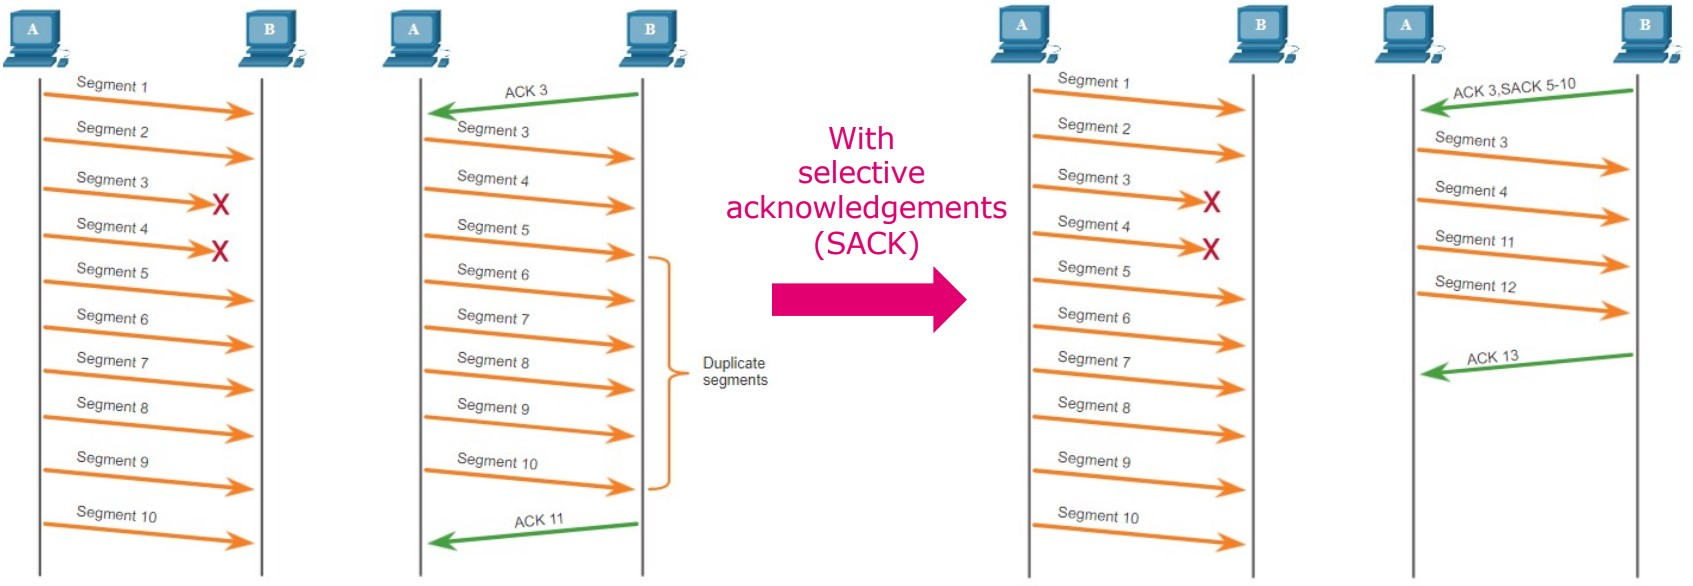
\includegraphics[width=\textwidth]{images/Selective_Acknowledgement.jpg}
    \caption{Datenverlust und nochmaliges Versenden (\textsuperscript{\textcopyright}Cisco)}
    \end{center}
\end{figure}